\section{Taxonomía}

Se ha desarrollado una cantidad significativa de trabajo en el área de 
pronóstico a muy corto plazo de secuencias espaciotemporales. Dado que 
el pronóstico de tormentas eléctricas está intimamente relacionado con el 
pronóstico de secuencias espaciotemporales este capítulo presentará una 
taxonomía de enfoques de pronóstico de secuencias espaciotemporales a muy 
corto plazo.\newline
La taxonomía presentada en la figura \ref{fig:taxonomia} en forma de árbol, 
dividida en dos ramas principales para las categorías de enfoques utilizados. 
Cada una de estas ramas es dividida en subcategorías de enfoques utilizados. 
Cada enfoque utilizado es subidividido en métodos utilizados.

\begin{figure}[H]
  \centering
  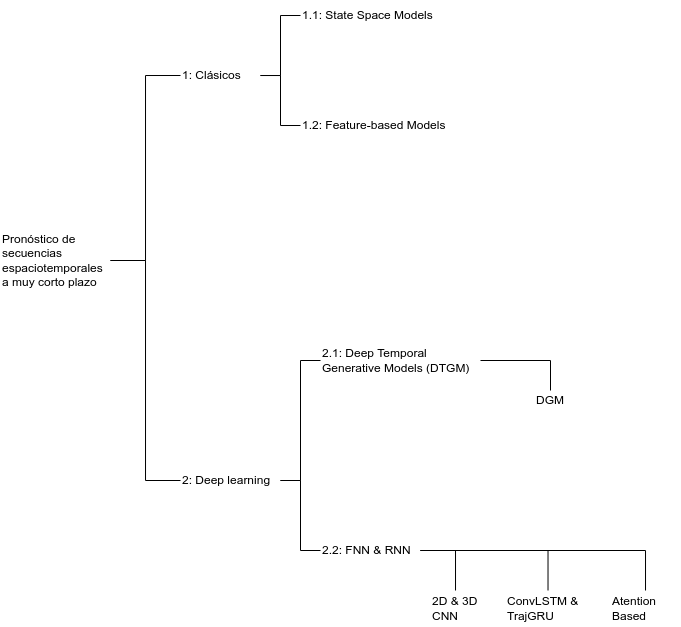
\includegraphics[width=14cm]{./E_IMAGENES/3_EstadoArte/taxonomia}
  \caption{
    Una taxónomía de los enfoques aplicados a la predicción de secuencias 
    espaciotemporales a muy corto plazo. Categorías extraidas de 
    \cite{DBLP:journals/corr/abs-1808-06865}.
  }
  \label{fig:taxonomia}
\end{figure}

El foco del presente trabajo está en el uso de técnicas de deep learning, por 
lo que no se realizaron mayores subdivisiones en los métodos clásicos.

\subsection{Enfoques Clásicos}
Dado que una secuencia espaciotemporal puede ser vista como una secuencia 
multivariada, los métodos diseñados para el pronóstico de series de tiempo 
multivariadas son aplicables a secuencias espaciotemporales.

\subsubsection{State Space Models}
Los Modelos de Espacio de Estados (State Space Models, SSM) analiza a las 
secuencias desde un punto de vista generativo, donde cada observación $X_t$ se 
asume generada por un estado oculto $H_t$ y esos estados ocultos forman un 
proceso de Markov. Ejemplos notables de este tipo de modelos son los 
Autoregressive Integrated Moving Average Model (ARIMA).

\subsubsection{Feature-based Models}
Los modelos basados en características resuelve el pronóstico de secuencias 
espaciotemporales al entrenar un modelo de regresión basado en características 
diseñadas por humanos.

\subsection{Enfoques Deep Learning}
Los enfoques de deep learning propuestos para el modelamiento de secuencias 
espaciotemporales aprovechan las capacidades de generalización de las redes
neuronales profundas.

\subsubsection{Deep Temporal Generative Models}
Los Modelos Generativos Profundos son modelos estadísticos que aprenden 
distribuciones de probabilidad de los datos y permiten facil generación de 
muestras de sus distribuciones aprendidas.

\begin{itemize}
  \item \textbf{DGM}: \cite{Ravuri2021} propuso el uso de Redes Generativas 
  Adversariales (Generative Adversarial Network, GAN) para modelar datos de 
  precipitación de radares meteorológicos en Reino Unido. El modelo propuesto 
  busca resolver el problema de pronósticos difuminados aprovechando la 
  capacidad de las GAN para generar pronósticos feasibles a cualquier plazo a 
  futuro.
  \begin{figure}[H]
    \centering
    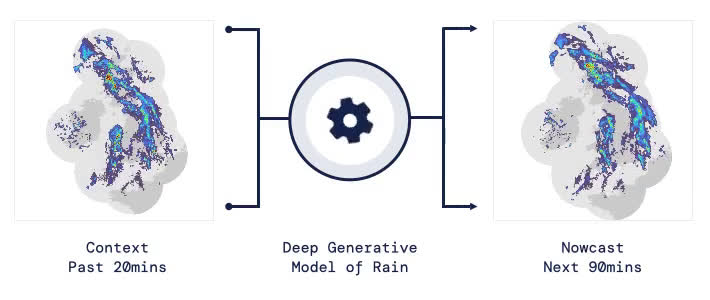
\includegraphics[width=8cm]{E_IMAGENES/3_EstadoArte/dgmr_1}
    \caption{
      Modelo de pronóstico de lluvia a muy corto plazo utilizando Redes 
      Generativas Adversariales. Fuente: \cite{Ravuri2021}
    }
    \label{fig:dgmr_modelo}
  \end{figure}
\end{itemize}

\subsubsection{FNN \& RNN}
\begin{itemize}
  \item \textbf{2D \& 3D CNN}: \cite{Cintineo2020} propuso el uso de Redes 
  Neuronales Convolucionales para pronósticar la probabilidad de convección 
  intensa. Su trabajo fue complementado con la explicabilidad de los 
  pronósticos, descubriendo los factores más significativos en el resultado del 
  modelo.
  \begin{figure}[H]
    \centering
    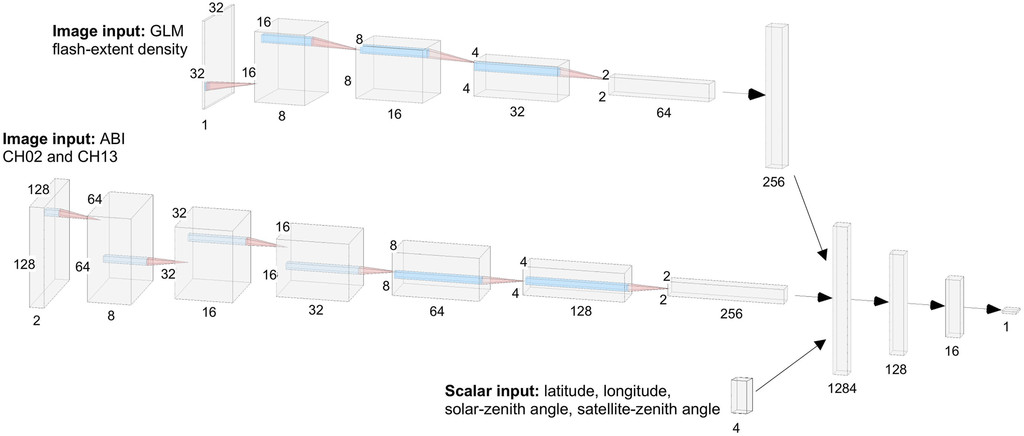
\includegraphics[width=10cm]{E_IMAGENES/3_EstadoArte/cintineo_1}
    \caption{
      Arquitectura de redes neuronales convolucionales para el pronóstico de 
      convección intensa. Fuente: \cite{Cintineo2020}.
    }
    \label{fig:cintineo}
  \end{figure}
  \cite{Chang2018} propuso el uso de datos topográficos para mejorar el 
  desempeño un modelo de pronóstico de precipitación, obteniendo mejor 
  desempeño que el modelo inicial, sin embargo, la proporción de falsa alarma 
  también se incrementó. Este artículo propone la incorporación de información 
  topográfica usando un bloque de convolución y max pooling como se observa en 
  la figura \ref{fig:chang}
  \begin{figure}[H]
    \centering
    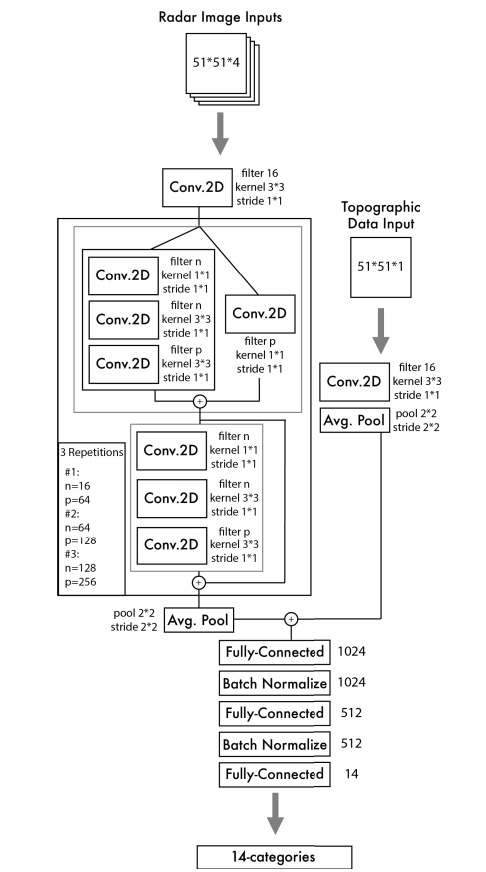
\includegraphics[width=8cm]{E_IMAGENES/3_EstadoArte/chang_1}
    \caption{
      Arquitectura de redes neuronales convolucionales que incorpora datos 
      topográficos. Fuente: \cite{Chang2018}.
    }
    \label{fig:chang}
  \end{figure}

  \item \textbf{ConvLSTM \& TrajGRU}: \cite{DBLP:journals/corr/ShiCWYWW15} 
  propuso una arquitectura de redes neuronales que combina la capacidad de 
  capturar correlación espacial de las CNN y la capacidad de capturar 
  correlación temporal de las LSTM, la denominó ConvLSTM. Las ConvLSTM utilizan 
  un estado oculto multidimensional para poder capturar información espacial y 
  actualizan sus estados por medio de la operación de convolución. 
  \begin{figure}[H]
    \centering
    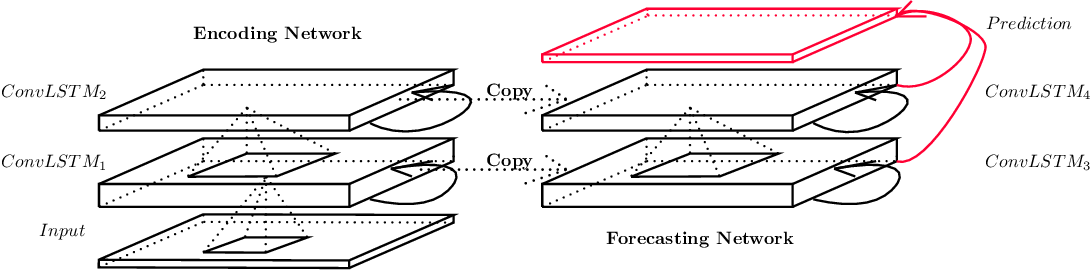
\includegraphics[width=8cm]{E_IMAGENES/3_EstadoArte/convlstm}
    \caption{
      Arquitectura de red neuronal convolucional LSTM para el pronóstico 
      inmediato de precipitación. Fuente: \cite{DBLP:journals/corr/ShiCWYWW15}.
    }
    \label{fig:convlstm}
  \end{figure}
  \cite{DBLP:journals/corr/ShiGL0YWW17} evaluó el desempeño de distintos 
  modelos de pronóstico inmediato para precipitación y propuso una nueva 
  arquitectura que resolvería el problema de la falta de sensibilidad a la 
  rotación de la arquitectura ConvLSTM, la denominó TrajGRU.
  \begin{figure}[H]
    \centering
    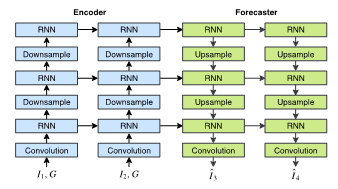
\includegraphics[width=8cm]{E_IMAGENES/3_EstadoArte/trajgru}
    \caption{
      Arquitectura de red neuronal Trajectory GRU para el pronóstico 
      inmediato de precipitación. Fuente: \cite{DBLP:journals/corr/ShiGL0YWW17}.
    }
    \label{fig:trajgru}
  \end{figure}

  \item \textbf{Atention based}: \cite{DBLP:journals/corr/abs-2003-12140} 
  propuso una arquitectura que utilice el mecanismo de atención para poder 
  capturar correlaciones temporales a largo plazo, la denominó MetNet. Su 
  arquitectura presentada en la figura \ref{fig:metnet} entrega como salida 
  distribuciones de probabilidad de precipitiación con un desempeño que supera 
  a los modelos actualmente empleados. El modelo cuenta con 225M parámetros 
  entrenables, por lo que su entrenamiento y despliegue requiere de un enorme 
  poder computacional.
  \begin{figure}[H]
    \centering
    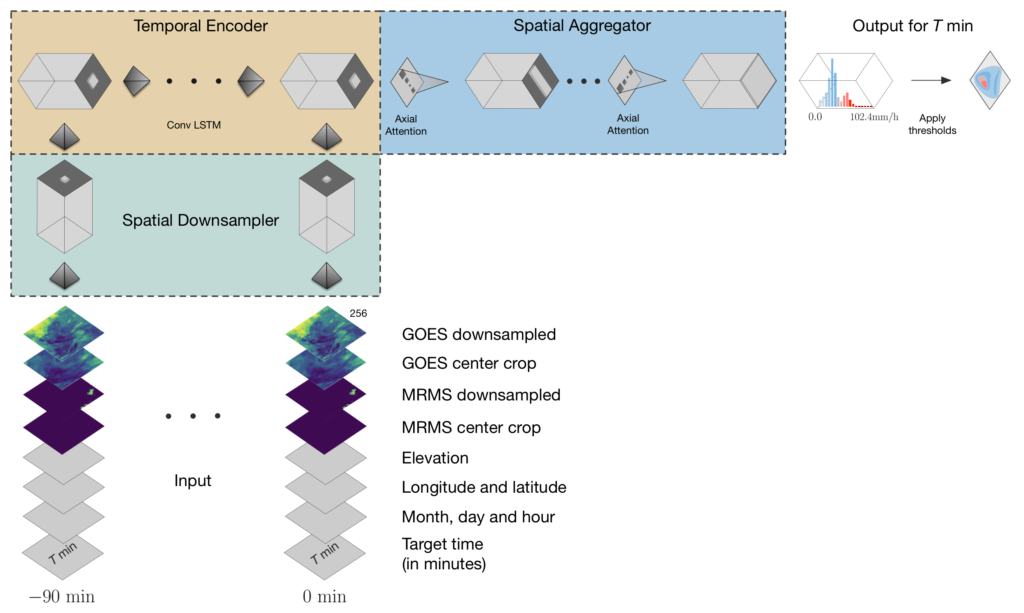
\includegraphics[width=12cm]{E_IMAGENES/3_EstadoArte/metnet}
    \caption{
      Arquitectura de red neuronal MetNet. Fuente: 
      \cite{DBLP:journals/corr/abs-2003-12140}.
    }
    \label{fig:metnet}
  \end{figure}

\end{itemize}


